% ALGUNOS PAQUETES REQUERIDOS (EN UBUNTU): %
% ========================================
% %
% texlive-latex-base %
% texlive-latex-recommended %
% texlive-fonts-recommended %
% texlive-latex-extra %
% texlive-lang-spanish (en ubuntu 13.10) %
% ******************************************************** %

\documentclass[a4paper]{article}
\usepackage[utf8]{inputenc}
\usepackage{fancyhdr}
\usepackage[pdftex]{graphicx}
\usepackage{sidecap}
\usepackage{caption}
\usepackage{subcaption}
\usepackage{booktabs}
\usepackage{makeidx}
\usepackage{float}
\usepackage{array}
\usepackage{amsmath, amsthm, amssymb}
\usepackage{amsfonts}
\usepackage{sectsty}
\usepackage{wrapfig}
\usepackage{listings}
\usepackage{pgfplots}
\usepackage{enumitem}
\usepackage{hyperref}
\usepackage{listings}
\usepackage{listingsutf8}
\usepackage{pgfplotstable}
\usepackage{colortbl}
\usepackage[spanish,es-nodecimaldot]{babel}

\linespread{factor}

\definecolor{mygreen}{rgb}{0,0.6,0}
\definecolor{mygray}{rgb}{0.5,0.5,0.5}
\pgfplotsset{compat=1.3}
\setlist[enumerate]{label*=\arabic*.}
\lstset{
	inputencoding=utf8/latin1,
	language=C++,
	basicstyle=\ttfamily,
	keywordstyle=\bfseries\color{blue},
	stringstyle=\color{red}\ttfamily,
	commentstyle=\color{mygreen}\ttfamily,
	morecomment=[l][\color{magenta}]{\#},
	numbers=left,
	numberstyle=\color{mygray}
}
\pgfplotstableset{% global config, for example in the preamble
  every head row/.style={before row=\toprule,after row=\midrule},
  every last row/.style={after row=\bottomrule},
  fixed,precision=2,
}

\usepackage{color} % para snipets de codigo coloreados
\usepackage{fancybox}  % para el sbox de los snipets de codigo

\definecolor{litegrey}{gray}{0.94}

% \newenvironment{sidebar}{%
% 	\begin{Sbox}\begin{minipage}{.85\textwidth}}%
% 	{\end{minipage}\end{Sbox}%
% 		\begin{center}\setlength{\fboxsep}{6pt}%
% 		\shadowbox{\TheSbox}\end{center}}
% \newenvironment{warning}{%
% 	\begin{Sbox}\begin{minipage}{.85\textwidth}\sffamily\lite\small\RaggedRight}%
% 	{\end{minipage}\end{Sbox}%
% 		\begin{center}\setlength{\fboxsep}{6pt}%
% 		\colorbox{litegrey}{\TheSbox}\end{center}}

\newenvironment{codesnippet}{%
	\begin{Sbox}\begin{minipage}{\textwidth}\sffamily\small}%
	{\end{minipage}\end{Sbox}%
		\begin{center}%
		\vspace{-0.4cm}\colorbox{litegrey}{\TheSbox}\end{center}\vspace{0.3cm}}



\usepackage{fancyhdr}
\pagestyle{fancy}
%\renewcommand{\chaptermark}[1]{\markboth{#1}{}}
\renewcommand{\sectionmark}[1]{\markright{\thesection\ - #1}}
\fancyhf{}
\fancyhead[LO]{Sección \rightmark} % \thesection\
\fancyfoot[LO]{\small{Nicolás Bukovits, Kevin Frachtenberg, Julián Len, Nicolás Len}}
\fancyfoot[RO]{\thepage}
\renewcommand{\headrulewidth}{0.5pt}
\renewcommand{\footrulewidth}{0.5pt}
%\setlength{\hoffset}{-0.8in}
\setlength{\textwidth}{16cm}
\setlength{\hoffset}{-1.1cm}
\setlength{\headsep}{0.5cm}
\setlength{\textheight}{25cm}
\setlength{\voffset}{-0.7in}
\setlength{\headwidth}{\textwidth}
\setlength{\headheight}{13.1pt}
\renewcommand{\baselinestretch}{1.1} % line spacing

\usepackage{caratula}

\newcommand{\ord}{\ensuremath{\operatorname{O}}}
\newcommand{\nat}{\ensuremath{\mathbb{N}}}

\begin{document}

\setcounter{page}{1}
\materia{Algoritmos y Estructuras de Datos III}
\submateria{Segundo Cuatrimestre de 2016}
\titulo{Trabajo Práctico I}
%\subtitulo{Grupo: }
\integrante{Nicolás Bukovits}{516/14}{nicobuk@gmail.com}
\integrante{Kevin Frachtenberg}{217/14}{kevinfra94@gmail.com}
\integrante{Julián Len}{467/14}{julianlen@gmail.com}
\integrante{Nicolás Len}{819/11}{nicolaslen@gmail.com}
\maketitle
% no footer on the first page
\thispagestyle{empty}

\newpage
\tableofcontents

\newpage
\section{Introducción}

En este trabajo se tienen tres problemas que se resolvieron aplicando las
técnicas algorítmicas estudiadas en la materia. Los mismos presentaron cada uno un desafío
distinto, teniendo que aplicar métodos diferentes para resolverlos y cumplir
con los requisitos exigidos.

Además de la resolución de los mismos, se procedió a demostrar la correctitud de
cada implementación. Esto fue acompañado a su vez de una justificación de la
complejidad temporal.

Cada ejercicio contó con su respectiva experimentación para corroborar que la
complejidad temporal teórica se cumpliera y en los casos donde el algoritmo
podía comportarse mejor, verlo reflejado de alguna manera.

Los experimentos contaron con diversas medidas para asegurar su efectividad de
las cuales las siguientes fueron iguales para los tres problemas:
\begin{itemize}
	\item{Sólo se midió el costo temporal de generar la solución, no
			de lectura y escritura del problema.}
	\item{Para la medición del tiempo se utilizó la biblioteca \texttt{chronos}
			con unidad de tiempo en nanosegundos.}
	\item{Todas las pruebas se ejecutaron en los laboratiorios de la facultad.}
\end{itemize}


\newpage
 \section{Ejercicio 1}
    % 1. Describir detalladamente el problema a resolver dando ejemplos del mismo y sus soluciones.
    \subsection{Descripción del problema}
		\begin{figure}[ht]
			\begin{center}
				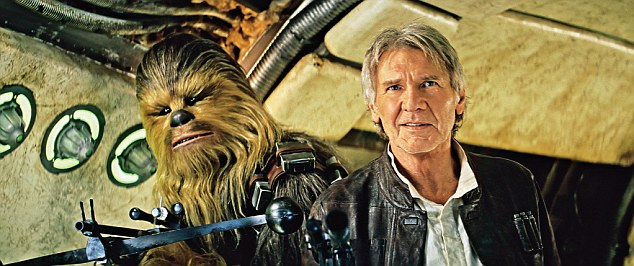
\includegraphics[width=0.5\columnwidth]{imagenes/expedicionistas.jpg}
				\caption{Indiana Jones junto a un Canibal del grupo de exploración}
			\end{center}
		\end{figure}
        Indiana Jones debe seguir un mapa que posiblemente lo lleve a encontrar la solución a P=NP. Para esto, lleva a un grupo de arquéologos compuesto por $A$ personas y le pide ayuda a un grupo de gente local de tamaño $C$ para poder llegar hasta su destino sin grandes problemas. Sin embargo, durante el camino se encuentran con un puente en mal estado en el que no podrán pasar más de dos personas a la vez. Sumado a eso, hay solo una linterna para todo el equipo, por lo que en cada cruce alguien debe volver con la linterna. Como si el problema del puente fuera poco, el grupo local es conocido por su canibalismo, así que no pueden quedar más caníbales que arqueólogos de alguno de los lados del puente.

        La resolución del problema consiste en elaborar un programa que recibe como entrada el valor de $A$ y $C$, y luego las velocidades de cada arqueólogo ($a_0, ... , a_A$) y la de cada canibal ($c_0, ... , c_C$) y devuelve la velocidad mínima con la que se puede cruzar el puente.

        Por ejemplo, si el programa recibe lo siguiente como entrada: \newline
        \texttt{2} \texttt{1} \newline
        \texttt{1} \texttt{2} \newline
        \texttt{1}

        La salida correcta sería: \newline
        \texttt{4}

    % 2. Explicar de forma clara, sencilla, estructurada y concisa, las ideas desarrolladas para la resolución del problema. Utilizar pseudocódigo y lenguaje coloquial (no código fuente). Justificar por qué el procedimiento resuelve efectivamente el problema.
    \subsection{Solución propuesta}
        La solución de este problema fue lograda considerando todos las formas de cruzar el puente suponiendo que de esa forma se pueda llegar a un final válido. Dado que el fin es cruzar de la forma más rápida, dejamos de lado quién va a cruzar el puente y nos enfocamos en a qué grupo pertenece. Siguiendo esta idea, siempre cruzarán los más rápidos de los que tengan la posibilidad de cruzar. Nos aseguramos de no perder casos en los que el cruce de alguien que no sea el más rápido nos lleve a una mejor solución basandonos el principio de optimalidad y en la idea de que todos deben cruzar el puente al menos una vez. El tiempo que les toma cruzar cada vez que pasan dos personas es la del más lento. Entonces, en el caso de que deba cruzar una sola persona, si hay dos del mismo grupo, será mejor que cruce el más rápido primero ya que en caso de tener que regresar, tendrá menos posibilidades de retrasar al acompañante. En el caso de que dos personas deban cruzar, podemos tomar la misma idea y cuando alguno deba volver a cruzar, deberá regresar el más rápido nuevamente para consumir la menor cantidad posible de tiempo (siempre y cuando cruce el del grupo que corresponda).

        Solamente van a tener la chance de cruzar quienes estén del lado en que está en la linterna y que su cruce no lleve a un \emph{estado inválido}. Un estado válido es aquél en el que no se estuvo anteriormente (es decir, que sea una situación que no haya ocurrido con anterioridad) y que no deje a más caníbales que arqueólogos de alguno de los dos lados. Si bien lo mejor es que crucen siempre los más rápidos, esto no siempre será posible. Es por esto, que los que crucen el puente serán los más rápidos de todas las combinaciones posibles entre los dos grupos siendo un cruce de 1 o 2 personas. Luego, los posibles cruces serán 2 personas del mismo grupo, 1 de un grupo y 1 de otro, o 1 sola de alguno de los dos grupos. Aquí es donde entra la importancia del estado inválido. La forma de corroborar que el movimiento lleve a un estádo válido es observando la cantidad de personas pertenecientes a cada uno de los grupos en cada lado del puente, sin importar su velocidad.

        La razón de esto es que es lo mismo si los que están en algún lado del puente son los que poseen velocidad $a_1$ o $a_2$ ya que simplemente sería una permutación de éstos. A pesar de que esto puede impactar en el tiempo total del cruce del puente, el objetivo de probar con todos los caminos y obtener todos las \emph{soluciones válidas} hace que luego no sea importante quién está de cada lado.

        Para que una solución al problema sea válida, el tiempo que tome cruzar el puente debe ser mayor o igual a la suma de las velocidades de los todos los exploradores (caníbales y arqueólogos) y además en ningún momento del recorrido deben haber estados inválidos. Además, se pide que la solución final sea el menor tiempo posible que tome cruzar el puente. Este mismo será el mínimo entre todas las soluciones válidas.

        Teniendo en cuenta lo planteado en este informe sobre el problema, podemos marcar que el algoritmo realizado, fue construido en base a la técnica de \emph{backtracking} que al igual que en este caso, consiste en probar todas las posibilidades descartando la mayor cantidad de soluciones incorrectas posibles al mismo tiempo y dejando como resultado una lista con las soluciones válidas. Así, se prueban todos los caminos posibles para cruzar el puente y al final se obtiene una lista con todas los tiempos que puede tomar cruzar el puente.

        Los casos base de la recursión son triviales, ya que resultan del cruce del puente de 1 o 2 exploradores, sin importar su grupo, y el tiempo que toma eso es la velocidad del más lento. Aquí solo pueden ocurrir casos inválidos cuando habiendo 2 exploradores, se intente realizar el cruce de solo uno de ellos. En cualquier otro caso, el cruce será de un solo cambio de estado y en ningún momento pueden haber más exploradores de algúno de los grupos.

        Para el caso recursivo, se chequeará antes de entrar en la recursión que el estado al que se va a cambiar sea uno válido. Si no lo es, cambia la cantidad de exploradores que vayan a cruzar. Si siguen obteniéndose estados inválidos, entonces no quedarán casos para probar y simplemente terminará la búsqueda en esa rama de estados sin haber encontrado una solución válida.

        \subsubsection{Detalles implementativos}
            El algoritmo fue implementado en lenguaje C++. Para almacenar la solución, se recurre a la clase \texttt{vector}, proporcionada por la librería estándar del lenguaje.

            Para manejar los estados en el árbol de ejecución, se van almacenando los nuevos estados en un vector de \texttt{Estados} antes de entrar en una recursión y se quita al retornar de la misma. Esto es para que en la misma altura del arbol haya la misma cantidad de estados y para que no haya estados inválidos de una rama de desiciones en otra en la que se tomaron otros caminos.

            Un \texttt{Estado} es una clase la cual consiste de 4 \texttt{Int}, 2 para la cantidad de arqueólogos y 2 para la cantidad de caníbales de cada uno de los lados en ese momento, y de un \texttt{Bool} para indicar si la linterna se encuentra a la derecha o no.

            Llamamos \emph{árbol de ejecución} al árbol que se va generando de acuerdo a las desiciones tomadas en cuanto a qué explorador cruzará el puente.

            La forma en que se elige quiénes cruzarán de un lado a otro luego de haber decidido a qué grupo pertenecen, es simplemente tomar los primeros (1 o 2) valores del vector que contiene a los arqueólogos o caníbales que vayan a pasar. De esta forma se están tomando siempre los más rápidos, como se mencionó anteriormente, ya que en cada iteración los 4 vectores de personas se ordenan de menor a mayor.

        \begin{codesnippet}
        \begin{verbatim}
si estadoActual tiene linterna a la derecha
  lado de origen  = lado derecho
  lado de destino = lado izquierdo
si no
  lado de origen  = lado izquierdo
  lado de destino = lado derecho
linternaEnDeracha = !linternaEnDerecha

ordenarVelocidades canibalesEnOrigen
ordenarVelocidades canibalesEnDestino
ordenarVelocidades arqueologosEnOrigen
ordenarVelocidades arqeuologosEnDestino

para #CanibalesQueCruzan entre 0 y minimo(2, #canibales del lado de origen):
    para #ArqueologosQueCruzan entre 0 y (2 - #CanibalesQueCruzan):
        si esEstadoValido(#CanibalesEnOrigen - #canibalesQueCruzan,
                          #ArqueologosEnOrigen - #arqueologosQueCruzan,
                          #CanibalesEnDestino + #CanibalesQueCruzan,
                          #ArqueologosEnDestino + #ArqueologosQueCruzan,
                          linternaEnDerecha, estadosAnteriores):

            canibalesQueCruzan = canibalesEnOrigen[0 hasta #CanibalesQueCruzan]
            agregar canibalesQueCruzan a CanibalesEnDestino
            eliminar canibalesQueCruzan de CanibalesEnOrigen

            arqueologosQueCruzan = arqueologosEnOrigen[0 hasta #ArqeueologosQueCruzan]
            agregar arqueologosQueCruzan a ArqueologosEnDestino
            eliminar arqueologosQueCruzan de ArqueologosEnOrigen

            nuevoEstado = (tamaño(ArqueologosEnOrigen),
                          tamaño(ArqueologosEnDestino),
                          tamaño(CanibalesEnOrigen),
                          tamaño(CanibalesEnDestino),
                          linternaEnDerecha)

            nuevoTiempo = tiempoActual + max(si mandarArqueologos > 0
                                               entonces maximo(arqueologosMasRapidos)
                                               sino 0,
                                             si mandarCanibales > 0
                                               entonces maximo(canibalesMasRapidos)
                                               sino 0)

            agregar nuevoEstado a EstadosAnteriores
            recursiónCruzarPuente(estadosAnteriores, nuevoTiempo, soluciones)
            eliminar nuevoEstado de EstadosAnteriores
        fin si
    fin para
fin para
        \end{verbatim}
        \end{codesnippet}

            Esta es una porción del algoritmo completo, en la cual se muestra cómo funciona la parte recursiva del mismo. La variable \emph{soluciones} no se modifica en esta parte ya que es simplemente agregar el tiempoActual a la lista, siendo tiempoActual el contador de tiempo que toma hasta ese estado cruzar el puente. La idea de agregar nuevoEstado a EstadosAnterirores consiste en poder eliminar los caminos que lleven a una situación que ya se haya estado con anterioridad (por ejemplo, que cruce un canibal y luego vuelva). Además, al quitarla luego de la recursión hace que para cada altura del árbol de ejecución tengamos la misma cantidad de estados y que éstos sean todos distintos. La razón por la cual serán distintos proviene de que cada estado se arma basándose en la cantidad de arqueólogos y caníbales que hay de cada lado y de qué lado está la linterna. Entonces si cada vez que haya que cruzar el puente se elige una cantidad distinta de exploradores, cada nuevo estado tendrá como máximo 5 formas distintas (que cruce un solo canibal, un solo arqueólogo, dos canibales, dos arqueólogos o un arqueólogo y un canibal).

            La otra parte importante del algoritmo consiste en chequear si lograron cruzar todos los exploradores, que en tal caso como se menciona en el párrafo anterior, se agrega el tiempo que tomó cruzar el puente. Luego, se regresa hacia arriba en un nivel en el árbol de ejecución y se continúa probando las otras posibilidades de caminos.



    % 3. Deducir una cota de complejidad temporal del algoritmo propuesto y justificar por qué el algoritmo cumple la cota dada. Utilizar el modelo uniforme.
    \subsection{Complejidad teórica}

      El algoritmo comienza tomando $2$ vectores, siendo uno para los arqueólogos y otro para los caníbales. En cada posición de cada uno se encontrará una velocidad correspondiente a algún arqueólogo o caníbal. El tamaño de cada vector será igual a la cantidad de arqueólogos/caníbales que se tomaron como entrada. Llamaremos $n$ a la cantidad de arqueólogos. Además, dada la lógica del algoritmo, si hay más caníbales que arqueólogos al comenzar, la ejecución termina sin llamar a la función principal y devuelve $-1$ inmediatamente, ya que no hay forma de que al comienzo haya más aqrueólogos que caníbales en el lado izquierdo. En cambio, si hay $0$ aqrueólogos o más arqueólogos que caníbales, sí se llama a la función que realiza \emph{Backtracking}.
      En ella, se utilizandolizan $2$ vectores más para poder distinguir el lado del que se encuentra cada arqueólogo y cada caníbal. La inserción y eliminación de cada elemento en cada vector será de $O(1)$ amortizado ya que en caso de que el vector deba redimencionarse, se copian todos los elementos del vector a uno más grande dejando como complejidad $O(n)$.
      En cada llamada a la función principal del algoritmo, se prueban $5$ casos: que cruce un arqueólogo solo, un canibal solo, dos arqueólogos, dos caníbales o un caníbal y un arqueólogo. Luego, cada nodo del árbol tendrá 5 hijos. Cada uno de ellos, será un posible estado válido y si lo es, se realizarán las operaciones necesarias para decidir quién cruzará el puente, las cuales consisten en los movimientos de personas entre vectores (que toma complejidad $O(n)$), previamente habiendo ordenado cada vector (en $O(n $log$ n)$) y luego llamar recursivamente a la función principal, lo que da una complejidad de $O(n $log$ n)$ para las operaciones que no son la llamada recursiva. Dado que se quieren probar todos los estados válidos, podemos decir que la complejidad temporal será el tiempo que tome recorrer cada uno de estos estados, que a la vez equivalen a los nodos del árbol de ejecución. Sabemos que la altura del árbol está acotada por la cantidad total de estados válidos. Este número se calcula de la siguiente manera:

      Dado que la cantidad de caníbales está acotada por la cantidad de arqueólogos, la cantidad de formas válidas que hay para repartir a todas las personas en ambos lados del puente manteniendo el invariante de que no haya más caníbales que arqueólogos de ninguno de los dos lados se calcula utilizando combinatoria. La cantidad de caníbales posibles en cada lado del puente es menor o igual a la cantidad de arqueólogos de ese lado (o sea entre $0$ y $n$), pero en caso de que no haya arqueólogos en alguno de los lados, la cantidad de caníbales posibles es igual a la cantidad total de arqueólogos, salvo que no haya ninguno y en ese caso $n$ pasará a ser el número de caníbales totales.

      \[
      \sum_{i=1}^{n}(i+1) + (n+1)
      \]
      \[
      \frac{(n+2)(n+1)}{2} + (n+1) - 1
      \]
      \[
      \frac{(n+2)(n+1)}{2} + n
      \]
      \[
      \frac{(n+2)(n+1)+2n}{2}
      \]
      \[
      \frac{n^2+3n+2}{2}
      \]

      Y de este tipo de funcion sabemos \newline

      \[
      \frac{n^2+3n+2}{2} \in O(n^2)
      \]

      Entonces, la altura del árbol va a estar acotada por $O(n^2)$.
      Retomando, llegamos a que la complejidad de encontrar las soluciones está acotada por $O(b^h)$ donde $b$ es la cantidad de ramas que se abren en cada nodo, $h$ es la altura del árbol y todo esto es el tamaño del árbol. Como mencionamos anteriormente, $b$ es exactamente $5$ y la altura del árbol está acotada por $O(n^2)$. Luego, la complejidad temporal para encontrar las soluciones sería $O(5^{n^2})$. Pero hasta aquí no tenemos en cuenta que cada nodo cuesta $O(n $log$ n)$. Incorporando esto a la complejidad anterior en la cual suponíamos que cada nodo tenía costo $O(1)$, nos queda que la complejidad temporal en peor caso es $O((n$ log $n) * 5^{n^2})$.

      En cuanto a la complejidad espacial, se utiliza un historial de estados anteriores en los que se van guardando los estados válidos por los que se pasó hasta cierto punto en cada nodo del árbol. Se usa como si fuera una pila y cada vez que se accede a un nivel inferior en el árbol de ejecución, se guarda el estado actual de los caníbales, los arqueólogos y la linterna; mientras que cuando se sube en el árbol, se elimina el último estado actual. Debido a esto, la complejidad espacial en es $O(n^2)$ ya que la pila tendrá a lo sumo el mismo tamaño que la cantidad de estados en la rama más larga, y como probamos antes, este valor está acotado por esa complejidad. Además, lo que se guarda en cada estado son 4 valores enteros que indican la cantidad de arqueólogos y caníbales de cada lado, y un booleano (representado con 1 o 0) que indica de qué lado está la linterna.


    % 4. Dar un código fuente claro que implemente la solución propuesta. Se deben incluir las partes relevantes del código como apéndice del informe impreso entregado.

    % 5. Realizar una experimentación computacional para medir la performance del programa implementado. Usar un conjunto de casos de test en función de los parámetros de entrada, con instancias aleatorias e instancias particulares (de peor/mejor caso en tiempo de ejecución, por ejemplo). Presentar en forma gráfica una comparación entre los tiempos medidos y la complejidad teórica calculada y extraer conclusiones.
    \subsection{Experimentación}

	Para poder acercarnos lo más posible a la cota propuesta en la complejidad temporal, realizamos experimentos con la mayor cantidad posible de personas sin que se extienda demasiado el tiempo de solución. Los casos de prueba pueden observarse en la siguiente tabla:

  %CORRER ./TP1 1 -EXP
  %LUEGO GRAFICAR, Y SUBIR EL CSV A http://www.tablesgenerator.com/latex_tables#

  \begin{table}[]
\centering
\caption{My caption}
\label{my-label}
\begin{tabular}{llll}
\hline
\multicolumn{1}{|l|}{\textbf{Tiempo en ms}} & \multicolumn{1}{l|}{\textbf{\#canibales}} & \multicolumn{1}{l|}{\textbf{\#arqueologos}} & \multicolumn{1}{l|}{\textbf{\#personas}} \\ \hline
11                                          & 0                                         & 1                                           & 1                                        \\
10                                          & 0                                         & 2                                           & 2                                        \\
20                                          & 0                                         & 3                                           & 3                                        \\
29                                          & 0                                         & 4                                           & 4                                        \\
41                                          & 0                                         & 5                                           & 5                                        \\
14                                          & 1                                         & 1                                           & 1                                        \\
62                                          & 1                                         & 2                                           & 2                                        \\
280                                         & 1                                         & 3                                           & 3                                        \\
1170                                        & 1                                         & 4                                           & 4                                        \\
4256                                        & 1                                         & 5                                           & 5                                        \\
0                                           & 2                                         & 1                                           & 1                                        \\
83                                          & 2                                         & 2                                           & 2                                        \\
431                                         & 2                                         & 3                                           & 3                                        \\
5510                                        & 2                                         & 4                                           & 4                                        \\
102579                                      & 2                                         & 5                                           & 5                                        \\
0                                           & 3                                         & 1                                           & 1                                        \\
0                                           & 3                                         & 2                                           & 2                                        \\
159                                         & 3                                         & 3                                           & 3                                        \\
1659                                        & 3                                         & 4                                           & 4                                        \\
116050                                      & 3                                         & 5                                           & 5                                        \\
0                                           & 4                                         & 1                                           & 1                                        \\
0                                           & 4                                         & 2                                           & 2                                        \\
0                                           & 4                                         & 3                                           & 3                                        \\
100                                         & 4                                         & 4                                           & 4                                        \\
2280                                        & 4                                         & 5                                           & 5                                        \\
0                                           & 5                                         & 1                                           & 1                                        \\
0                                           & 5                                         & 2                                           & 2                                        \\
0                                           & 5                                         & 3                                           & 3                                        \\
0                                           & 5                                         & 4                                           & 4                                        \\
128                                         & 5                                         & 5                                           & 5                                        \\ \hline
\end{tabular}
\end{table}

	\begin{itemize}
		\item{Como entrada se utilizó $N = k$ con $200 < k < 100000$}
		\item{Por cada $N$, se repitió 40 veces la medición y se calculó un
			promedio.}
	\end{itemize}

	De estos puntos, cabe destacar la elección de comenzar con $N = 200$. Esta
	decisión surge del hecho de que en valores pequeños las mediciones de tiempo
	son más sensibles a perturbaciones del sistema en el que están corriendo.
	Por lo tanto, en base a las pruebas realizadas, se optó por ignorar los
	primeros valores dado que no aportaban información pertinente al experimento.

	Los resultados obtenidos fueron los siguientes. En los gráficos, $T$ representa el
    tiempo de ejecución obtenido en las mediciones.

	\newcommand\constante{3}
	\begin{figure}[H]
		\centering
		\caption{}
		\label{fig:exp1:tiempo_base}
		\begin{tikzpicture}
			\begin{axis}[
					title={},
					xlabel={Tamaño de entrada ($N$)},
					ylabel={Tiempo de ejecución (nanosegundos)},
					scaled x ticks=false,
					scaled y ticks=false,
					enlargelimits=0.05,
					width=0.5\textwidth,
					height=0.5\textwidth,
					legend pos=south east,
					legend cell align=left,
					xmin=1
				]
				\addplot[color=black] table[x index=0,y index=1]{../exp/kaioKenOutput};
				\addplot[color=red] table[x index=0, y expr={x*ln(x)*\constante}]{../exp/kaioKenOutput};
				\legend{$T$, $c*N*log(N)$}
			\end{axis}
		\end{tikzpicture}
	\end{figure}

	En la Figura \ref{fig:exp1:tiempo_base} se puede observar como la curva generada por el
	tiempo de ejecución puede ser acotada para un $c$ fijo por una función
	$c*N*log(N)$. Para ratificar esta observación se procede dividiendo cada $T$
	por su respectivo $N$ con la intención de generar una curva de forma
	logarítmica.

	\begin{figure}[H]
		\centering
		\caption{}
		\label{fig:tiempo_sobre_n}
		\begin{tikzpicture}
			\begin{axis}[
					title={},
					xlabel={Tamaño de entrada ($N$)},
					ylabel={Tiempo de ejecución (nanosegundos)},
					scaled x ticks=false,
					scaled y ticks=false,
					ymax=100,
					enlargelimits=0.05,
					width=0.5\textwidth,
					height=0.5\textwidth,
					legend pos=south east,
					legend cell align=left,
					xmin=1
				]
				\addplot[color=black] table[x index=0,y index=2]{../exp/kaioKenOutput};
				\addplot[color=red] table[x index=0, y expr={ln(x)*\constante}]{../exp/kaioKenOutput};
				\legend{$\frac{T}{N}$, $c*log(N)$}
			\end{axis}
		\end{tikzpicture}
	\end{figure}

	Con la Figura \ref{fig:tiempo_sobre_n} se corrobora lo previsto, ya que
	efectivamente se puede apreciar cómo con la misma constante $c$ se puede
	acotar por una función $c*log(N)$.

	\begin{figure}[H]
		\centering
		\caption{}
		\label{fig:tiempo_sobre_n_log_n}
		\begin{tikzpicture}
			\begin{axis}[
					title={},
					xlabel={Tamaño de entrada ($N$)},
					ylabel={Tiempo de ejecución (nanosegundos)},
					scaled x ticks=false,
					scaled y ticks=false,
					ymin=0,
					ymax=5,
					enlargelimits=0.05,
					width=0.5\textwidth,
					height=0.5\textwidth,
					legend pos=south east,
					legend cell align=left,
					xmin=1
				]
				\addplot[color=black] table[x index=0,y index=3]{../exp/kaioKenOutput};
				\addplot[color=red] table[x index=0, y expr={\constante}]{../exp/kaioKenOutput};
				\legend{$\frac{T}{N*log(N)}$, $c$}
			\end{axis}
		\end{tikzpicture}
	\end{figure}

	Finalmente, en la Figura \ref{fig:tiempo_sobre_n_log_n} se tiene que
	$\frac{T}{N*log(N)}$ converge a una constante que puede ser acotada por $c =
	\constante$. Este $c$ es el mismo que es utilizado en las figuras
	anteriores.

	Es así como se llega a la conclusión de que efectivamente la complejidad
	temporal de la solución desarrollada coincide con la complejidad teórica estipulada.

	Para reproducir los datos utilizados basta con ejecutar \texttt{KaioKenSolver
	-p}.


\newpage

\section{Ejercicio 2: Problemas en el camino}
    % 1. Describir detalladamente el problema a resolver dando ejemplos del mismo y sus soluciones.
	\subsection{Descripción del problema}

	\begin{figure}[ht]
		\begin{center}
			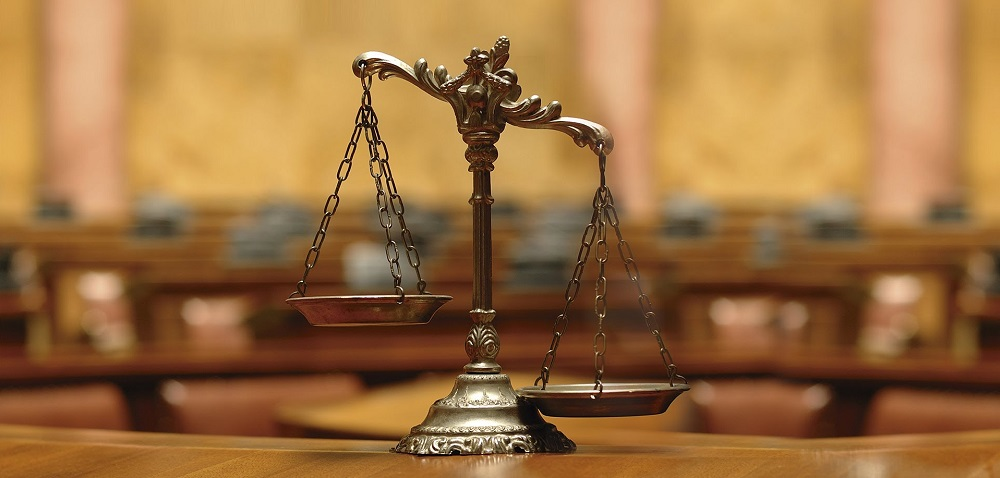
\includegraphics[width=0.5\columnwidth]{imagenes/balanza.jpg}
			\caption{Equilibro}
		\end{center}
	\end{figure}

	Luego de cruzar el puente, el equipo se encuentra en una habitación amplia con una puerta, la cual está cerrada. En el medio de la habitación hay una balanza de dos platillos, la cual contiene sobre su platillo izquierdo una llave que abre la puerta de la habitación. Al retirar la llave, se cambia el equilibro de la balanza, lo cual hace que se cierre la entrada de la habitación. La llave no sirve para abrir la puerta y lo único que puede realizar el equipo es recompener el equilibro de la balanza utilizando un conjunto de pesas de potencia de 3 distintas. Es decir, sólo disponen de una sóla pesa de cada potencia de 3. Los datos de entrada y de salida para el problema son los siguientes: 

	~

	\textbf{Formato de entrada:} El único dato de entrada es un entero $P$ que representa el peso de la llave.

	\begin{tabular}{ll}
		\texttt{P}
	\end{tabular}

	~

	\textbf{Salida:} La salida consiste en dos enteros $S$ y $T$ que representan la cantidad de pesas que hay que colocar en el platillo izquierdo y el derecho respectivamente, seguidas de otra línea con los valores de las pesas que se deben colocar del platillo izquierdo ordenadas de menor a mayor y finalmente otra línea con los valores de las pesas del platillo derecho, también con el mismo orden.

	\begin{tabular}{ll}
		\texttt{S} & \texttt{T} \\
		\texttt{I1 ...} & \texttt{...IS} \\
		\texttt{D1 ...} & \texttt{...DT} \\
	\end{tabular}

	~

	Se tiene como restricción que el peso $P$ está en el siguiente rango: 1$<=$ $P$ $<=$ $10^{15}$. La complejidad temporal debe ser a lo sumo $\ord(\sqrt{P})$. 

    % 2. Explicar de forma clara, sencilla, estructurada y concisa, las ideas desarrolladas para la resolución del problema. Utilizar pseudocódigo y lenguaje coloquial (no código fuente). Justificar por qué el procedimiento resuelve efectivamente el problema.
    \subsection{Solución propuesta}

	La idea propuesta para la resolución del problema consiste en buscar cómo obtener una representación del número $p$. Si se consigue una representación del mismo se puede equilibrar la balanza. Primero nos abtraemos de las restricciones del problema y pensamos que cualquier número $a$ $\in$ \mathds{N} admite un desarrollo en base $d$, utilizando sólo símbolos comprendidos en el rango de 0 a $d-1$. Como se dispone de sólo pesas que son potencias de 3, se decide utilizar la base 3 para representar el número. Si el problema no tuviera la restricción de que sólo se dispone de una pesa de cada potencia de 3, la resolución sería trivial ya que sólo consiste en obtener el desarrollo en base 3 del número $p$ (que es un dato de entrada y que se asume que su desarrollo es en base 10) y poner tantas pesas de cada potencia de 3 (hasta 2 por potencia ya que en base 3, sólo se pueden utilizar los símbolos 0, 1 y 2) como indique el desarrollo, en el plato de la izquierda de la balanza para obtener el mismo peso $p$. Pero la restricción de que sólo se dispone de una sóla pesa de cada potencia de 3 hace que dicha solución no funcione. No obstante, teniendo en cuenta que en la balanza, las pesas que se colocan en el lado derecho 'restan' el peso colocado en el plato izquierdo se puede pensar en una solución en la cual cuando se tengan que utilizar dos pesas de la misma potencia, se puedan reemplazar por el uso de una pesa mayor colocada en el plato izquierdo (la cual se interpretaría como suma de dicha potencia de 3) y el uso de otra pesa colocada en el plato derecho (la cual se interpretaría como resta de dicha potencia de 3). Para lograr que la suma de dicha pesa menos la resta de la otra pesa, den como resultado el mismo valor que las dos pesas originales, se debe encontrar alguna relación entre las potencias de 3. La solución propuesta consiste en lo siguiente: 

	\newline

     \textbf{Caso 1:} El desarrollo en base 3 del número $p$ no contiene el símbolo 2.

    Este caso es trivial. Significa que a lo sumo se usa una vez cada potencia de 3 en el desarrollo del número. Por lo tanto, para obtener la solución al problema sólo bastar tomar las pesas correspondientes (las potencias de 3 que se utilizan en el desarrollo) y colocarlas en el plato izquierdo de la balanza para obtener el mismo peso original $p$ y equilibrarla.

	\newline

     \textbf{Caso 2:} El desarrollo en base 3 del número $p$ contiene al menos un símbolo 2.

    Este es el caso interesante ya que no se dispone de dos pesas de la misma potencia. Sin embargo, se pueden reemplazar dos pesas de la misma potencia de la siguiente manera:

    \newline

    \begin{center}

    	2.3^n = 3^{n+1} - 3^{n}

    	\newline

		2.3^n = 3.3^n - 3^n

		\newline

		2.3^n = (3 -1).3^n

		\newline

		2.3^n = 2.3^n

    \end{center}

	Es decir, se pueden reemplazar dos pesas de una potencia de 3 por la inmediata potencia de 3 superior menos una sóla pesa de las dos potencias de 3. Igualmente esto no siempre se puede realizar ya que puede darse el caso de que ya se estén usando dos pesas de la potencia de 3 inmediata superior como en el siguiente ejemplo:  


    \newline
    \begin{center}

    	$p$ = 1.3^2 + 2.3^1 + 2.3^0
    
    \end{center} 

    Entonces se debe encontrar una solución general que resuelva el problema antes mencionado. Se propone la siguiente solución:

    \newline
    \begin{center}

    \sum_{i=0}^{n}2.3^i = 3^{n+1} - 3^i

    \end{center}

    Se realiza la demostración de la anterior fórmula usando inducción en $n$: 

   \newline
    \textbf{Caso base:} $n = 0$

    \newline
    \begin{center}
    
    \sum_{i=0}^{0}2.3^i = 3^{1} - 3^0

    \newline

    2.3^0 = 3 - 1

	\newline

    2 = 2
    \end{center} 

    \newline
    \textbf{Paso inductivo:} Usamos como hipótesis inductiva (HI) que la fórmula vale para $n$ y queremos probar que vale para $n + 1$.

    \newline
    \begin{center}

    \sum_{i=0}^{n+1}2.3^i = 3^{n + 2} - 3^i

    \newline
    \sum_{i=0}^{n}2.3^i + 2.3^{n+1} = 3^{n + 2} - 3^i

    \newline
    Por HI:

    3^{n+1} - 3^i + 2.3^{n+1} = 3^{n + 2} - 3^i

   	\newline
	3.3^{n+1} - 3^i = 3^{n + 2} - 3^i

   	\newline
	3.3.3^{n} - 3^i = 3^{2}.3^{n} - 3^i

   	\newline
	9.3^{n} - 3^i = 9.3^{n} - 3^i

    \end{center} 

	\begin{flushright}

	\Box
	\end{flushright}

    Como conclusión se puede observar que cuando se tenga el caso de que no sea posible tomar una pesa de una potencia de 3 porque ya se usan dos pesas de dicha potencia y tampoco sea posible reemplazarla por la siguiente ya que también se usan dos pesas de dicha potencia (es decir, en el desarrollo del número hay varios símbolos 2 consecutivos) se debe buscar la primer potencia de 3 más grande de la cual no se tenga que utlizar dos pesas y reemplazar las pesas originales por la suma del valor de la potencia 3 de la pesa encontrada menos el valor de la potencia de 3 más chica de la cual se utilizan dos pesas. Esta fórmula se puede aplicar a cada uno de los símbolos en el desarrollo del número.


	\subsubsection{Implementación}\label{ej2_imp}

	Habiendo introducido la idea, se detalla el comportamiento del algoritmo para
	una entrada con $P$.

	Se presenta un pseudocódigo para tener de referencia al seguir la
	explicación detallada a continuación:

	\begin{codesnippet}
	\begin{verbatim}
	izquierda = verdadero
	divisiones = 0
	izquierdas = []
	derechas = []
	Mientras p != 0
	    cociente = p / 3
	    resto = p - (cociente *3)
	    Si resto es 0
	      Si no lo puse en izquierda al anterior
	        Agrego a izquierdas la pesa con valor (3 ^ divisiones)
	      izquierda = verdadero
	    Si resto es 1
	      Si anterior lo puse en izquierda
	        Agrego a izquierdas la pesa con valor (3 ^ divisiones)
	      Si no
	        Agrego a derechas la pesa con valor (3 ^ divisiones)
	    Si resto es 2
	      Si anterio lo puse en izquierda
	        Agrego a derechas la pesa con valor (3 ^ divisiones)
	      izquierda = falso
	    p = cociente
	    divisiones += 1
	Fin Mientras
	Si el último no lo puse en la izquierda
	   Agrego a izquierdas la pesa con valor (3 ^ divisiones)
	\end{verbatim}
	\end{codesnippet}

	\begin{enumerate}
		\item{
			La primera parte consiste en la inicialización de valores para el algoritmo. Se tiene una variable booleana que indica en qué platillo fue colocada la última pesa para cada iteración. Esta variable se inicializa en verdadera y es utilizada para saber en qué platillos hay que colocar las pesas que siguen. Esta variable es muy importante ya que determina en qué casos se van a reemplazar dos pesas de una potencia de 3, por otras pesas y cómo hacerlo. La variable divisiones es simplemente un índice que representa la cantidad de divisiones realizadas al número P. Por último se tienen dos listas inicializadas vacías, que van a almacenar las pesas que hay que colocar en los platillos izquierdo y derecho.
		}

		\item{
			El ciclo principal se ejecuta mientras P sea distinto de cero. En el cuerpo del ciclo se realiza la división del número P por 3 y se almacenan en dos variables distintas el cociente y el resto de dicha operación. Para el caso del valor del resto se tienen 3 posibilidades:
			\begin{enumerate}
				\item{
					EL resto es igual a 0: En este caso hay que preguntar si la anterior pesa fue colocada o no en el platillo derecho. Si fue colacada en el platillo derecho, se agrega a la lista de izquierdas la pesa que corresponde al valor (3$^{divisiones}$). La variable izquierda se actualiza con el valor verdadero, indicando que la última pesa fue colacada del lado izquierdo.
				}
				\item{
					El resto es igual a 1. En este caso tenemos dos posibilidades distintas:
					\begin{enumerate}
						\item{
							La anterior pesa fue colocada del lado izquierdo, por lo tanto esta pesa también tiene que colocarse del mismo lado. Se agrega entonces a la lista de izquierdas el valor (3$^{divisiones}$).
						}
						\item{
							La anterior pesa fue colocada del lado derecho, por lo tanto esta pesa también tiene que colocarse del mismo lado. Se agrega entonces a la lista de derechas el valor (3$^{divisiones}$).
						}
					\end{enumerate}
				\item{
					El resto es igual a 2: Sólo basta con fijarse si la anterior pesa fue colacada en el platillo izquierdo. De ser así, se debe agregar a derechas la pesa con el valor (3$^{divisiones}$).
				}
				}
				\end{enumerate}
			}
			\item{
			    Lo último que se realiza en el ciclo es actualizar el valor de P, el cual va a contener el valor del cociente calculado al principio. De esta manera el valor de P se irá decrementando en cada ciclo hasta llegar a cero. También se suma uno al índice de divisiones.
				Finalmente, se pregunta si la última pesa fue colocada en la lista de derechas. De ser así, se agrega a la lista de izquierdas la pesa con valor (3$^{divisiones}$).
			}
	\end{enumerate}

	\subsubsection{Demostración de correctitud}

	Habiendo visto cómo funciona el algoritmo desarrollado, se procede a
	justificar por qué devuelve una solución. Para esto se explicará el algoritmo en base a las justificaciones matemáticas realizadas en la solución propuesta.
	\subsubsection*{Correctitud de ciclo}

	Lo que se va a demostrar a continuación es que el ciclo principal termina y calcula la solución al problema.

	El ciclo se ejecuta mientras P sea distinto de cero. Es decir termina cuando P es 0 y esto ocurre ya que lo que se hace en el ciclo es dividir el número P por 3 y reemplazar P por el resultado (cociente) de esta división en cada iteración. Eventualmente el cociente va a ser cero, por los teoremas de división entera y de desarrollo en base $d$. Lo que se está haciendo es utilizar el algoritmo de división para obtener el desarrollo en base 3 del número $P$. Los restos en cada iteración son los que indican que símbolos hay que utilizar para la representación del número en esa base. En este caso no interesa obtener la representación del número en base 3, sino trabajar con los símbolos en su desarrollo (restos). El resto de la división sólo puede ser 0, 1 o 2 (por el teorema de la división entera).

	A continuación se analiza la parte fundamental del algoritmo que consiste en la identificación de qué pesas utilizar y en qué platillos colocarlas dependiendo del resto. Se tienen las siguientes posibilidades: 

	\begin{enumerate}
		\item{
			Resto == 0. En este caso, si la última pesa fue colocada del lado izquierdo no hay que realizar nada. Esto es porque el anterior dígito en el desarrollo era o bien otro cero o un 1. Por lo tanto no es necesario utilizar esta pesa para compensar una de un valor menor que no pudo ser utilizada porque se estaban usando dos (esto fue explicado en la solución propuesta). En cambio si la anterior pesa fue colocada del lado derecho es porque el anterior dígito en el desarrollo del número era un 2. En este caso, hay que utilizar esta pesa, por lo que se agrega a la lista de izquierdas el valor de la potencia de 3 correspondiente. Independientemente de si se utilizó esta pesa o no, la variable izquierda se actualiza con el valor verdadero, ya que el hecho de que no se use una pesa de una determinada potencia también se toma como que se 'usó'' la pesa de la izquierda. Esto es porque en el caso de que el siguiente dígito en el desarrollo sea un uno, se tiene que poder distinguir si el anterior fue un 0 o un 2, lo cual no se podría realizar si no se actualiza el valor de esta variable. En la explicación del caso del resto 1 se puede entender mejor esta conclusión. 
		}
		\item{
			Resto == 1. En este caso siempre hay que agregar una pesa. Si el valor de la variable izquierda es verdadero (esto es porque el anterior dígito fue un 0 o un 1) hay que agregar esta potencia de 3 a la lista de izquierda. En el caso contrario significa que el anterior dígito era un 2 y como se demostró en la solución propuesta hay que colocar esta pesa en el lado derecho, ya que si el anterior fue un 2 hay que tomar este dígito, lo que lo convertiría de un 1 a un 2, y por lo tanto hay que aplicar nuevamente la fórmula propuesta. Por lo tanto en este último caso se agrega la potencia de 3 correspodiente en la pesa derecha. El valor de la variable izquierda no es necesario actualizarlo ya que si se agrega a la lista de izquierdas hay que modificarlo por verdadero (lo cual ya ocurre porque se agrega solamente a izquierdas si es verdadero) y si se agrega a la lista de derechas hay que modificarlo por falso (lo cual ya ocurre porque se agrega solamente a derechas si es falso).
		}
		\item{
			Resto == 2. En este caso se usa también la idea planteada en la solución al problema. Se agrega a la lista de derechas la pesa con el valor de la potencia de 3 correspondiente solamente si la anterior fue colocada en el lado izquierdo (es decir el anterior dígito es un cero o un uno) ya que si el anterior era un 2 no hay que realizar nada (por lo visto en la demostración de la solución). Finalmente se actualiza el valor de izquierda y se pone en falso siempre, ya que es necesario para el siguiente dígito en el desarrollo, ya que como se vió si el siguiente es cero va a haber que tomar la siguiente pesa y si es un 1 va a haber que colocar la pesa en el lado derecho.	
		}
	\end{enumerate}

	Como el ciclo finaliza cuando P es igual a cero, se puede dar el caso de que el último dígito en el desarrollo del número en base 3 (el más significativo) sea un 2. Por lo tanto y sabiendo que no sigue ningún dígito más, lo que hay que hacer si se da este caso es tomar esta pesa por lo visto en la solución.

	En conclusión lo que hace el algoritmo es dividir iterativamente el número por 3, obteniendo de esta forma su desarrollo en base 3 y al mismo tiempo colocando las pesas correspondientes en base a los restos obtenidos (teorema de desarrollo en base $d$). No es necesario obtener primero la representación del número en la base y después aplicar la solución; se puede realizar mientras se obtiene, tomando decisiones en base al resto de la división en cada iteración. La idea propuesta garantiza que el algoritmo siempre va retornar una solución por lo visto en la sección de "Solución". Las decisiones que se toman con los restos son las inferidas por la solución propuesta: si el dígito es 0, no se toma esa pesa salvo que el anterior sea un 2. si el dígito es 1, si el anterior es 0 o 1 se toma esa pesa, sino se resta la pesa; finalmente si el dígito es 2, si anterior es 2 no se toma ninguna acción y si no se resta la pesa. Además el algoritmo de división garantiza que las pesas que se toman, van a estar ordenadas de menor a mayor cumpliendo con la restricción del problema.

    % 3. Deducir una cota de complejidad temporal del algoritmo propuesto y justificar por qué el algoritmo cumple la cota dada. Utilizar el modelo uniforme.
	\subsection{Complejidad teórica}

	Para calcular la complejidad teórica de la solución propuesta se hará
	referencia a la sección \ref{ej2_imp} donde se posée el pseudocódigo junto a
	su explicación.

	El algoritmo tiene una complejidad temporal de $\ord(log(n))$, por lo tanto es
	logarítmico y cumple con la restricción de complejidad del enunciado. Esto se justifica con el hecho de que el algoritmo posee un ciclo
	principal que se ejecuta mientras $P$ sea distinto de cero, es decir desde el número $P$ hasta el número 0. En cada iteracion el tamaño de $P$ se reduce a un tercio, ya que se divide por 3. Por lo tanto el ciclo se ejecuta la cantidad de símbolos necesarios para obtener el número $P$ en base 3. Si $P$ requiere de $n$ símbolos es que:

	\newline
	$d^{n-1} <= P < d^n$

	\newline
	es decir, $n -1 <= log_3(P) < n$, lo que implica que $[log_3(P)] = n - 1$ y por lo tanto $n = [log_3(P)] + 1$


	Dentro del ciclo sólo se hacen comparaciones que tienen un costo asociado de $\ord(1)$, una división, una multiplicación y una resta de enteros (costo $\ord(1)$), una asignación y una suma, y se agregan elementos a una lista (todas estas operaciones tambien en $\ord(1)$). Por lo tanto se concluye que la complejidad del ciclo es $\ord(log(n))$. Fuera del ciclo sólo se realizan incializaciones de variables $\ord(1)$ al principio del algoritmo y una comparación e inserción en una lista al final también en $\ord(1)$. Por álgebra de órdenes de funciones, la complejidad temporal resultante del algoritmo es $\ord(log(n))$. 

    % 4. Dar un código fuente claro que implemente la solución propuesta. Se deben incluir las partes relevantes del código como apéndice del informe impreso entregado.

    \subsection{Experimientacion}
         

	Se realizaron pruebas experimentales para verificar que el tiempo de
	ejecución del algoritmo cumpliera con la cota asintótica de $\ord(log(n))$,
	demostrada teóricamente. Para ello fue necesario modificar el algoritmo propuesto, ya que como la complejidad está definida por la cantidad de símbolos necesarios para la representación del número en base 3 y se explicó que la misma era $log_3$ del número más uno, no se observan grandes diferencias en el tiempo de ejecución para números 'razonables', es decir números que puedan ser representados de una forma práctica y eficiente en C++. Por ejemplo para el caso de un número muy grande como $3^{30}$, la cantidad de iteraciones que va a realizar el ciclo es sólo 31, que no es muy diferente a la cantidad de iteraciones necesarias para el número $3^{3}$ (4 iteraciones) que es mucho menor. Los tiempos de ejecución de estas instancias son muy similares y dado a que hay muchas variables en cuestión cuando se corren (otros procesos que interfieren, atención de interrupciones y scheduling del S.O, etc) puede hasta darse el caso de que tarde más una instancia menor que una mayor. Se presenta la siguiente modificación del algoritmo para realizar las pruebas:

	\begin{codesnippet}
	\begin{verbatim}
	izquierda = verdadero
	divisiones = 0
	izquierdas = []
	derechas = []
	Mientras v.size != 0
	    Si v[size -1] = 0
	      Si no lo puse en izquierda al anterior
	        Agrego a izquierdas la pesa con valor (3 ^ divisiones)
	      izquierda = verdadero
	    Si v[size -1] = 1
	      Si anterior lo puse en izquierda
	        Agrego a izquierdas la pesa con valor (3 ^ divisiones)
	      Si no
	        Agrego a derechas la pesa con valor (3 ^ divisiones)
	    Si v[size -1] = 2
	      Si anterio lo puse en izquierda
	        Agrego a derechas la pesa con valor (3 ^ divisiones)
	      izquierda = falso
	    v.size -= 1
	    divisiones += 1
	Fin Mientras
	Si el último no lo puse en la izquierda
	   Agrego a izquierdas la pesa con valor (3 ^ divisiones)
	\end{verbatim}
	\end{codesnippet}

	Este algoritmo a diferencia del original, recibe como parámetros un arreglo de enteros (v) que representa el desarrollo en base 3 de un número y un entero que es el tamaño del arreglo. El arreglo de enteros puede contener por lo tanto en cada posición un entero entre 0 y 2 inclusive. El arreglo se interpreta como que en la posición 0 está el dígito más significativo y en la última el menos significativo.
	Con esta idea se puede realizar un mejor análisis del rendimiento del algoritmo ya que se pueden simular números mucho más grandes. Se puede tomar un arreglo de 5000 posiciones, lo cual representaría un número muy grande en base 3 que no se puede representar directamente. La idea es que este algoritmo realiza en el fondo lo mismo que el anterior, ya que lo que se hace es recorrer el arreglo (ciclo principal) y después tomar las mismas decisiones que en el original en base a los valores contenidos en cada posición del arreglo. Es decir lo que determina la complejidad en este caso es el tamaño del arreglo, pero el mismo por lo expuesto anteriormente es igual al logaritmo en base 3 de un número P cualquiera, el cual sería el resultante de realizar la descomposición del desarrollo.

	Para las pruebas lo que se realizó es probar con arreglos de tamaño 1 hasta 4600. Para estandarizar y que no haya constantes diferentes para cada arreglo (ya que lo que se hace depende del valor de cada posición) en todos los casos se completaron todas las posiciones de los arreglos con el valor 1, para que el tiempo esté determinado sólo por el tamaño del arreglo. Además cada uno de los arreglos es testeado 5000 veces para disminuir los outliers. Lo esperable es que haya una relación lineal entre el tiempo de corrida y el tamaño del arreglo, pero el mismo se debe interpretar como que la relación es logarítmica entre el número que representa el arreglo y el tiempo.Se utilizó para que esto se visualice mejor la escala logarítica, como se puede observar en el siguiente gráfico:  


    \renewcommand\constante{5}

	\begin{figure}[H]
      \begin{center}
        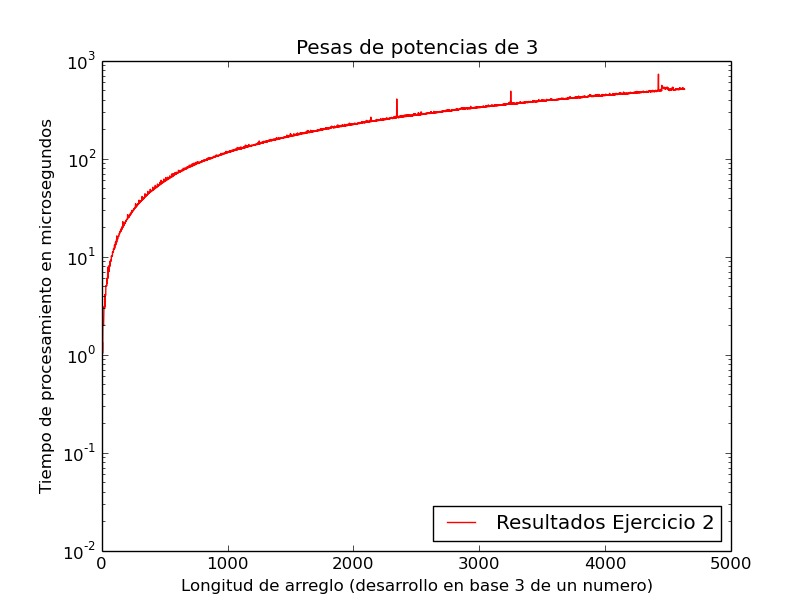
\includegraphics[width=0.7\columnwidth]{imagenes/ejercicio2.jpg}
        \caption{}
      \end{center}
  \end{figure}

El análisis expuesto de los datos recopilados presenta evidencia empírica sobre la cota de complejidad
demostrada teóricamente. Además se logra ver que la complejidad depende estrictamente de la cantidad
de símbolos que hay que utilizar para el desarrollo del número en base 3.

\newpage
\section{Ejercicio 3}
    % 1. Describir detalladamente el problema a resolver dando ejemplos del mismo y sus soluciones.
    \subsection{Descripción del problema}

		\begin{figure}[ht]
			\begin{center}
				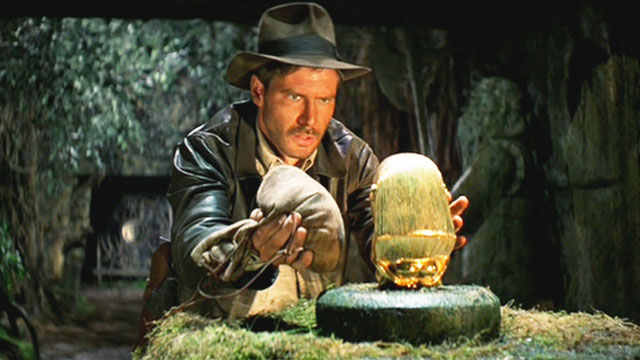
\includegraphics[width=0.4\columnwidth]{imagenes/tesoros.jpg}
				\caption{Fortuna y gloria muñeca, fortuna y gloria}
			\end{center}
		\end{figure}

        Una vez equilibrada la balanza, las paredes vuelven a su lugar. Con la llave obtenida logran abrir la puerta que estaba trabada. \par
		Al iluminar la habitación se encuentran con una sala de N tesoros. \par
		Por cada tipo de tesoro i, hay $C_{i}$ cantidades, con un valor $V_{i}$ y un peso $P_{i}$. Si bien el objetivo principal de la expedición era otro, nunca viene mal armarse de algún recuerdo. 
		Tienen M mochilas disponibles para llevarse los tesoros y cada una tiene una capacidad máxima de peso $K_{j}$ que puede llevar. \par
		El objetivo es llevarse el mayor valor posible de tesoros. Para esto, se debe devolver como resultado el valor total de tesoros guardados y además, por cada mochila, la cantidad de tesoros llevados y de qué tipo son.

        Por ejemplo, para la siguiente entrada:
        
        \begin{verbatim}
        M = 2
        K = { 1, 3 }
        
        N = 3 
        C = { 1, 2, 3 }
        V = { 2, 4, 10 }
        P = { 1, 2, 5 }
        \end{verbatim}

        Una posible salida válida sería:

        \begin{verbatim}
        S = 6
        M1 = { 1, 1 } 
        M2 = { 1, 2 }
        \end{verbatim}

        Es decir, para el caso en el que tenemos dos mochilas con capacidades 1 y 3, y nos encontramos con tres tesoros, el primero de peso 1 y valor 2, el segundo de peso 2 y valor 4, y el tercero de peso 5 y valor 10... \par Nos llevaremos en la primer mochila el primer tesoro y en la segunda el segundo tesoro. El tercer tesoro ya no nos entra.

    % 2. Explicar de forma clara, sencilla, estructurada y concisa, las ideas desarrolladas para la resolución del problema. Utilizar pseudocódigo y lenguaje coloquial (no código fuente). Justificar por qué el procedimiento resuelve efectivamente el problema.
    \subsection{Solución propuesta}
    Para solucionar el problema planteado se usó la técnica algorítmica de \emph{Programación dinámica}. \par
    La idea es separar el problema principal en subproblemas. En este caso, el subproblema es, en base a la capacidad restante de cada mochila y al valor y peso de cada tesoro, en qué mochila nos conviene meter cada uno (incluyendo la opción de no meterlo en ninguna). \par
    Por lo tanto, el algoritmo propuesto consta de una matriz por tesoro, de tamaño $(N+1)*(M+1)$ (suponiendo que hay dos mochilas), siendo éstas las capacidades de las mochilas $M_{1}$, $M_{2}$ respectivamente. Y además una matriz nula de igual dimensión que servirá para el caso en donde no hayan tesoros. \par
    El algoritmo funciona de la siguiente manera:
    1) Se crea una matriz de $M_{1}$ * $M_{2}$ para cada tesoro, y una extra inicial con los valores de todas las posiciones inicializados en 0.

    \begin{codesnippet}
    \begin{verbatim}
    for i = 1 .. cantTesoros + 1
        for j = 1 .. capacidadMochila1 + 1
            for k = 1 .. capacidadMochila2 + 1
                matriz[i][j][k] <-- 0
            end
        end
    end
    \end{verbatim}
    \end{codesnippet}

    2) Para cada posición (i, j) de la matriz del tesoro t, siendo i y j la capacidad \emph{restante} de la mochila 1 y 2, me fijo si t entra en alguna de las dos mochilas.
    Si entra en la mochila 1, obtengo valor(t) sumado al valor de la matriz del tesoro t-1 (recordar que el primer tesoro tiene una matriz predecesora con todos sus valores nulos) en la posición correspondiente según la capacidad restante de esa mochila (i - peso(t), j).
    Repito este procedimiento para cada mochila. 
    Y además me fijo el valor de la posición (i, j) de la matriz del tesoro t-1 para incluir el caso en el que no meto el objeto a la mochila.
    Luego me quedo con el resultado mayor de cada suma, y lo guardo en la matriz del tesoro t, en la posición (i, j)..

    \begin{codesnippet}
    \begin{verbatim}

    valorMochila1 = 0
    valorMochila2 = 0
    valorNingunaMochila = matriz[t-1][i][j]

    if pesoTesoro <= capacidadRestanteMochila1 then
        valorMochila1 <-- valor(t) + matriz[t-1][i - pesoTesoro][j]
    endif

    if pesoTesoro <= capacidadRestanteMochila2 then
        valorMochila2 <-- valor(t) + matriz[t-1][i][j - pesoTesoro]
    endif

    matriz[t][i][j] <-- max(valorMochila1, valorMochila2)

    \end{verbatim}
    \end{codesnippet}

    Repito este procedimiento para cada tesoro, hasta completar todas las posiciones de cada matriz.
    El último valor obtenido de la matriz del último tesoro, será el valor máximo que podemos acumular en las mochilas con los tesoros

    3) Luego, empezando desde la matriz del último tesoro, desde la última posición (i, j), me fijo en qué mochila entra ese tesoro... SEGUIR ACA



    El objetivo de hacer esto, es tener en cuenta todos los casos y valores acumulados, de poner o no cada tesoro, y en qué mochila se pone. Utilizando en todo caso el mayor valor de tesoros acumulados. En los campos de la matriz ira el valor que queda de poner el tesoro o no, y las capacidades restantes de las mochilas. \par
    El algoritmo se divide en dos partes, una parte es completar las matrices de tesoros, con el maximo valor posible que se puede acumular en cada mochila según el peso disponible. La segunda parte, consiste en definir, qué tesoros van en cada mochila, ubicando según el valor restante, de poner el tesoro en una mochila u otra.

    Para esto, uno puede pensarlo como una matriz de tres dimensiones o un cubo por tesoro, además de un cubo nulo. Por cada tesoro que se analiza, los pasos son iguales. Si la capacidad de las mochilas, representado por el índice (i,j,k) que las recorre (i representa la capacidad de la M1, j de la M2 y K de la M3) es menor que el peso del tesoro, el valor obtenido es igual al acumulado en el tesoro anterior (salvo el primer caso, en donde el tesoro anterior es la matriz nula). Si entra en alguna mochila, uno debe fijarse, que valor restante se obtiene, de restarle a su índice, el peso del objeto. Y, en la posición de la matriz se deja el máximo de ponerlo en alguna mochila o no ponerlo.\par

    Una vez explicado brevemente, pasaremos a detallar el algoritmo, dividiéndolo en dos secciones. La primera, completa las matrices de los tesoros, según el valor máximo posible por capacidad. Mientras que la segunda sección, recorre de atras para adelante las matrices, para ubicar los tesoros.\par

    El siguiente pseudocodigo mostrara como se completan las matrices,

    \begin{codesnippet}
	\begin{verbatim}
    cuboMagico = Inicializo un vector de matrices de Int
    Inicializo cantTesoros+1 matrices de (N + 1)*(M + 1)*(K +1) y las guardo en el vector cuboMagico.
    //N, M y K capacidades de las mochilas.
    for(iTesoroActual= 0...cuboMagico.size()) do
        //Recorro todas las matrices de tesoros
        iTesoro = El indice a la matriz del tesoro anterior.
        valorTesoro = tesoroValor[iTesoroActual]
        pesoTesoro = tesoroPeso[iTesoroActual]
        valorNingunaMochila = 0; //Me guardo el valor por si no entra en ninguna mochila
        //Recorro todas las matrices de tesoros
        for(iMochila1 = 0 .. N + 1) do
            for(iMochila2 = 0 .. M + 1) do
                for(iMochila3 = 0 .. N + 1) do
                    if(pesoTesoro entra en alguna mochila) do
                        if(pesoTesoro entra en mochila M_{1})
                            valorMochila1 = valorTesoro + cuboMagico[iTesoro][iMochila1-pesoTesoro][iMochila2][iMochila3]; 
                            //Valor de la matriz del tesoro anterior.
                        endif
                        if(pesoTesoro entra en mochila M_{2}) do
                    	    valorMochila2 = valorTesoro +  cuboMagico[iTesoro][iMochila1][iMochila2 - pesoTesoro][iMochila3];
                    	    //Valor de la matriz del tesoro anterior.
                        endif
                        if(pesoTesoro entra en mochila M_{3}) do
                            valorMochila3 = valorTesoro + cuboMagico[iTesoro][iMochila1][iMochila2][iMochila3 - pesoTesoro];
                            //Valor de la matriz del tesoro anterior.
                        endif
                    cuboMagico[iTesoro][iMochila1][iMochila2][iMochila3] = max(valorNingunaMochila, valorMochila1, valorMochila2, valorMochila3);
                    //Me quedo con el maximo de ponerlo en alguna mochila o no ponerlo.
                    iTesoro ++ //Avanzo el indice al tesoro anterior.
                end
            end
        end

	\end{verbatim}
	\end{codesnippet}






	Para la segunda parte, se decide por cada tesoro, en qué mochila irá. Para esto, se recorre desde la última posición de la matriz del último tesoro. En esta posición, se encuentra el mejor valor acumulado posible. La decisión se toma de la siguiente manera
		%Listita:
		 A) En qué mochilas entra?
		 B) Para cada mochila en la cual entra. Qué valor restante se encuentra en la posición de la matriz del del tesoro anterior en los pesos restantes, de ponerlo en cada una de las mochilas.
		 C) En el caso que el valor restante sea igual, lo pongo en cualquiera de las dos
		 D) En el caso que haya un máximo, ubico el tesoro en la mochila que obtiene el valor máximo restante.
	Sigo este algoritmo por cada matriz, hasta no tener capacidad disponible en ninguna de las mochilas.

	Si se analiza la forma en que se construye la solución, tanto en la primera como en la segunda etapa, se tienen en cuenta cuál es el valor máximo posible acumulado, de ubicar los tesoros. Es por esto que el resultado, siempre dará la suma máxima posible.

   

    \subsubsection{Detalles implementativos}
    
    El algoritmo fue implementado en lenguaje C++. Para almacenar la solución, se recurre a la clase \texttt{vector}, proporcionada por la librería estándar del lenguaje.

    Durante la ejecución del algoritmo se utilizan dos variables globales; un entero para almacenar la cantidad de enemigos y un vector que contiene la ubicación de cada uno de ellos. La ejecución consiste principalmente de una función recursiva, que presenta las siguientes características:

    \begin{itemize}
        \item Se prueban todos los pares de enemigos posibles mediante dos ciclos anidados, de la forma que se describe en el primer punto de la sección anterior.
        \item Dentro del ciclo interior se revisa a qué enemigos destruye el kamehameha descripto por el par de enemigos elegido y se destruyen esos enemigos para luego agregarlos a la solución.
        \item Destruir los enemigos consiste en eliminarlos de un vector que contiene a los enemigos restantes. Este vector es una copia del vector de enemigos restantes; el original debe conservarse porque, para cada kamehameha distinto, el algoritmo se bifurca con diferentes enemigos restantes.
        \item Agregarlos a la solución consiste en añadir un vector que contiene a dichos enemigos a un vector de vectores, que representa la solución parcial construida hasta el momento: cada posición del vector corresponde a un kamehameha distinto y contiene a los enemigos que el mismo destruye.
        \item Sus casos base son las llamadas donde la cantidad de enemigos restantes es igual o menor que 2. Estos casos no necesitan realizar llamadas recursivas, y simplemente devuelven un vector cuyo único enemigo es el vector de los enemigos a destruir, ya que estos pueden ser liquidados con un único kamehameha.
    \end{itemize}

    % hecho. Deducir una cota de complejidad temporal del algoritmo propuesto y justificar por qué el algoritmo cumple la cota dada. Utilizar el modelo uniforme.
    \subsection{Complejidad teórica}

    Al comienzo se inicializa un vector de $N$ posiciones, lo cual tiene costo del orden de $N$. El algoritmo consiste principalmente de una función recursiva, cuyo costo determina la complejidad temporal total de la solución.
    
    Dicha función contiene dos ciclos, un dentro del otro; el ciclo exterior recorre índices desde $0$ hasta $N - 1$, y el interior, desde $i$ hasta $N$. Esto implica que lo implementado dentro del ciclo interior se ejecute $N \times (N - 1)$ veces. Analizando este último ciclo, puede verse que:

    \begin{itemize}
        \item Se recorren todos los kamehamehas anteriormente lanzados, que a lo sumo pueden ser $N/2$, ya que cada kamehameha elimina al menos a 2 androides. Esto tiene un costo del orden de $N$.
        \item Se destruyen los enemigos alcanzados por el kamehameha. Esto consiste en recorrerlos todos (ciclo con orden de $N$ iteraciones) y borrar cada uno del vector donde estan almacenados (esto cuesta también $\ord(N)$), con un costo del orden de $N^2$. Luego se los agrega a un vector con enemigos destruidos, con un costo del orden de $N$. Por lo tanto, el costo total es del orden de $N^2$.
        \item Por último se llama a la misma función en forma recursiva.
    \end{itemize}

    Se debe observar que al hacer el nuevo llamado, la cantidad de enemigos va a haber disminuido al menos en 2. Debido a esto, dentro de la siguiente llamada, el ciclo exterior recorrerá solo $N - 2$ indices y el interior $N - 3$. Así estas cantidades disminuirán de a 2 hasta terminar, llegando a 1.

    %% IMPORTANTE: LLEGUÉ A REVISAR HASTA ACÁ.

    Si pensamos la cantidad de llamadas recursivas como un árbol donde cada node es una llamada, tenemos un árbol de a lo sumo $N/2$ niveles, donde en su primer nivel hay $N \times (N - 1)$ llamados. Cada uno tiene $(N - 2) \times (N - 3)$ hijos, a su vez cada uno de ellos $(N - 4) \times (N - 5)$ y así sucesivamente hasta llegar a 1. Por lo que en el segundo nivel habrán $N \times (N - 1) \times (N - 2) \times (N - 3)$ nodos, y de esta forma en el último nivel se encontraran $N!$ hojas.

    El árbol no puede tener más de $N/2$ niveles ya que cada nivel representa un kamehameha, y no pueden haber más de $N/2$ kamehamehas.

    Ejemplo para $N$ = 4: 

    \begin{center}
    \includegraphics[width=0.6\columnwidth]{imagenes/ej3_arbol.pdf}
    \end{center}
    
    Se puede ver como para el caso de $N = 4$ tenemos que la raiz tiene $4 \times 3 = 12$ hijos y que cada uno tiene $2 \times 1 = 2$ hijos. En otras palabras, en la primera ejecución (la raíz) se hacen 12 llamados (uno por cada par de enemigos), y para cada uno se hacen dos llamados (uno por cada par de enemigos restantes).

    En el nivel $k$ con $0 \leq k \leq N / 2$ se puede ver que cada nodo tiene $(N - 2k) \times (N - 2k - 1)$ hijos,
    debido a los ciclos explicados previamente. Entonces la cantidad de nodos en el nivel $k$ está dada por la cantidad de nodos en $k - 1$ multiplcado por $(N - 2k) \times (N - 2k -1)$. De esta forma la cantidad de nodos en el nivel $k$ es igual al producto de las cantidades de hijos por nodo de cada nivel, hasta $k$. Es decir, 

    \[\text{\#nodos en nivel }k = \prod_{l = 0}^{k}(N - 2l) \times (N - 2l -1)\]

    Y por lo tanto se cumple para el último nivel ($k = N/2$) donde los nodos son hojas

    \[\text{\#hojas }= \prod_{l = 0}^{N / 2}(N - 2l) \times (N - 2l -1) = N!\]

    Sabiendo que la cantidad de hojas es $N!$ y la altura es $N/2$, y que cada llamada tiene un costo de orden $N^2$, se puede pensar que este arbol de ejecución está acotado superiormente por una ``matriz'' de $N/2$ filas y $N!$ columnas donde cada elemento es una llamada de costo $N^2$.

    Es decir, la complejidad del algoritmo está acotada superiormente por $N/2 \times N! \times N^2$ que es de orden $N^3 \times N!$.

    Ahora veremos que vale $N^k \times N! \leq k! \times N^N$ $\forall k$ constante, particularmente lo vale para $k = 3$, y que por lo tanto $N^3 \times N!$ está acotado superiormente por $N^N$ que a su vez está acotado por $N^{N + 2}$, por lo que el algortimo cumple la complejidad requerida.

    \[ N^N = \prod_{i = 0}^{n - 1}n = N^k \times \prod_{i = 0}^{N - k - 1} N \geq N^k \times \prod_{i = 0}^{N - k - 1} (N - 1) = N^k \times \frac{N!}{k!}\]

    Dado que $N^N \geq N^k \times \frac{N!}{k!} \implies k! \times N^N \geq N^k \times N!$ y por lo tanto $N^k \times N! \in \ord(N^N) \forall k \in \nat$

    % 4. Dar un código fuente claro que implemente la solución propuesta. Se deben incluir las partes relevantes del código como apéndice del informe impreso entregado.

    % 5. Realizar una experimentación computacional para medir la performance del programa implementado. Usar un conjunto de casos de test en función de los parámetros de entrada, con instancias aleatorias e instancias particulares (de peor/mejor caso en tiempo de ejecución, por ejemplo). Presentar en forma gráfica una comparación entre los tiempos medidos y la complejidad teórica calculada y extraer conclusiones.
    \subsection{Experimentación}

        Al igual que con los otros dos ejercicios, se realizaron pruebas experimentales para verificar que el tiempo de ejecución del algoritmo cumpliera con la cota asintótica de $\ord(N^3 \times N!)$, teóricamente demostrada para el peor caso. Se realizaron dos tipos de pruebas:
        
        \begin{itemize}
            \item Pruebas con instancias con características particulares, más específicamente, para el mejor caso, el peor caso y casos intermedios.
            \item Pruebas con instancias generadas aleatoriamente, para obtener una aproximación al comportamiento del algoritmo en el caso promedio.
        \end{itemize}

        \subsubsection{Instancias particulares}

            Todas las instancias utilizadas para estas pruebas se generaron de manera aleatoria, pero restringiendo los resultados obtenidos para cumplir con determinadas características. A continuación se enumeran los criterios tenidos en cuenta para la generación de los escenarios de prueba.

            \begin{itemize}
                \item \textbf{Mejor caso:} El mejor caso del algoritmo se produce cuando todos los androides a destruir están ubicados sobre una única línea recta. En este caso, es seguro que el primer kamehameha con el que se intente será la solución óptima del problema, por lo que solo se bajará por esa rama de la recursión.

                \item \textbf{Peor caso:} El peor caso del algoritmo se da cuando no existen tres androides alineados a destruir. En consecuencia, cada kamehameha destruirá tan solo dos enemigos, que es el mínimo posible. Esto maximiza la complejidad temporal del algoritmo por dos motivos. Por un lado, en cada nivel de la recursión, se intentarán disparar todos los kamehamehas posibles, con la esperanza de que pueda encontrarse una solución más razonable. Por otra parte, en cada llamada recursiva que se efectúe, la entrada solo se reducirá en dos elementos, haciendo que la profundidad de la recursión alcance siempre la cota máxima de $\frac{N}{2}$.

                \item \textbf{Caso intermedio:} También se agregó un escenario de prueba adicional, con el objetivo principal de poner a prueba la efectividad de las podas implementadas. El mismo consiste en la combinación de dos instancias de mejor caso de tamaño $\frac{N}{2}$; es decir, la mitad de los androides se encuentran sobre una línea recta y la otra mitad, sobre una recta diferente. Las coordenadas de los enemigos son mezcladas de forma aleatoria para evitar que el kamehameha óptimo sea necesariamente el primero que se intente.
                
                Bajo estas condiciones, cabe esperar que las podas entren en acción, reduciendo considerablemente cantidad de llamadas recursivas que se ejecutan completas y consiguiendo un rendimiento apreciablemente superior al observado en el peor caso.

                Cabe destacar que este es un simple caso adicional de prueba, concebido con el objetivo de ilustrar la gran variación en el rendimiento del algoritmo según las características de los datos de entrada, pero que no guarda relación alguna con el comportamiento del algoritmo en el caso promedio.
            \end{itemize}

            Para los tres escenarios previstos, se generaron instancias de prueba para todos los valores de $N$ entre $1$ y $12$, inclusive. Luego, en cada caso, se ejecutaron $60$ repeticiones del algoritmo, midiendo cada vez el tiempo de ejecución y tomando luego el promedio entre los resultados obtenidos.

            En un principio, se descubrió que se producían picos en el tiempo de ejecución en las primeras corridas del programa, tendiendo los valores a estabilizarse con las sucesivas corridas. Si bien no se pudo determinar con precisión el origen de estas anomalías, se decidió, para minimizar la varianza de los datos obtenidos, tratar a las primeras $20$ repeticiones de cada instancia como \emph{outliers}, y promediar solo los valores de las últimas $40$.

            \renewcommand\constante{0.1}

            Los resultados obtenidos se exponen en el gráfico de la Figura \ref{fig:exp3:part_tiempo_base}, donde se ilustra también la cota teórica de $c \times N^3 \times N!$ (el valor de $c$ utilizado es \constante). Se representan como $T_P$ los tiempos obtenidos para peor caso, como $T_M$ para el mejor caso, y como $T_I$ para el caso intermedio. Puede observarse claramente que, incluso en el peor escenario, el tiempo de ejecución del algoritmo tiende a aumentar a un ritmo estrictamente más lento que el de la cota prevista.

            \begin{figure}[H]
                \centering
                \caption{}
                \label{fig:exp3:part_tiempo_base}
                \begin{tikzpicture}
                    \begin{axis}[
                            title={},
                            xlabel={Tamaño de entrada ($N$)},
                            ylabel={Tiempo de ejecución (nanosegundos)},
                            ymode = log,
                            scaled x ticks=false,
                            scaled y ticks=false,
                            enlargelimits=0.05,
                            width=0.5\textwidth,
                            height=0.5\textwidth,
                            legend pos=north west,
                            legend cell align=left,
                            xmin=1
                        ]

                        \addplot[color=red] table[x index=0,y index=1]{../exp/kamehamehaPeor};
                        \addplot[color=blue] table[x index=0,y index=1]{../exp/kamehamehaIntermedio};
                        \addplot[color=green] table[x index=0,y index=1]{../exp/kamehamehaMejor};
                        \addplot[color=gray] table[x index=0, y expr={\constante * (x^3) * x!}]{../exp/kamehamehaPeor};
                        \legend{$T_P(N)$, $T_M(N)$, $T_I(N)$, $c \times N^3 \times N!$}
                    \end{axis}
                \end{tikzpicture}
            \end{figure}

            En la Figura \ref{fig:exp3:part_tiempo_sobre_exp} se muestra el cociente entre los datos obtenidos y la función $N^3 \times N!$ (se considera el mismo valor de $c$ que en el gráfico anterior). Puede observarse como, al aumentar el tamaño de $N$, el cociente se aproxima rápidamente a $0$, ilustrando el hecho de que el crecimiento asintótico de la cota es estrictamente mayor que el de los tiempos obtenidos en las mediciones.

            \begin{figure}[H]
                \centering
                \caption{}
                \label{fig:exp3:part_tiempo_sobre_exp}
                \begin{tikzpicture}
                    \begin{axis}[
                            title={},
                            xlabel={Tamaño de entrada ($N$)},
                            ylabel={Tiempo de ejecución (nanosegundos)},
                            ymode = log,
                            scaled x ticks=false,
                            scaled y ticks=false,
                            enlargelimits=0.05,
                            width=0.5\textwidth,
                            height=0.5\textwidth,
                            legend pos=north west,
                            legend cell align=left,
                            xmin=1
                        ]

                        \addplot[color=red] table[x index=0,y expr={\thisrowno{1} / (x^(x+2))}]{../exp/kamehamehaPeor};
                        \addplot[color=blue] table[x index=0,y expr={\thisrowno{1} / (x^(x+2))}]{../exp/kamehamehaIntermedio};
                        \addplot[color=green] table[x index=0,y expr={\thisrowno{1} / (x^(x+2))}]{../exp/kamehamehaMejor};
                        \addplot[color=gray] table[x index=0, y expr={\constante}]{../exp/kamehamehaPeor};
                        \legend{$\frac{T_P(N)}{N^3 \times N!}$, $\frac{T_M(N)}{N^3 \times N!}$, $\frac{T_I(N)}{N^3 \times N!}$, $c$}
                    \end{axis}
                \end{tikzpicture}
            \end{figure}

            El análisis expuesto de los datos recopilados presenta evidencia empírica sobre la pertinencia la cota de complejidad demostrada teóricamente. Más aún, permite llegar a la conclusión que, incluso en las instancias de peor caso, esta cota resulta holgada, es decir, que la complejidad del algoritmo presentado es estrictamente $\ord(N^3 \times N!)$.

        \subsubsection{Instancias aleatorias}

            Para obtener una aproximación al comportamiento del algoritmo en el caso promedio, se realizaron también pruebas con instancias generadas de forma completamente aleatoria. Este experimento también se realizó para los valores de $N$ entre $1$ y $12$, y al igual que el anterior, la prueba se repitió $60$ veces para cada valor de $N$, descartando los resultados de las primeras $20$ repeticiones y promediando los obtenidos en las otras $40$. Sin embargo, esta vez cada medición se realizó sobre una instancia de prueba diferente, generada al azar.

            Intuitivamente, resulta razonable conjeturar que la probabilidad de que al tres enemigos se encuentren alineados en una instancia aleatoria es muy baja, especialmente teniendo en cuenta los pequeños tamaños de entrada considerados. En otras palabras, parece esperable que un escenario aleatorio tenga características similares a un escenario de peor caso, y por lo tanto, que el rendimiento promedio del algoritmo sea similar a este último caso.

            En la figura \ref{fig:exp3:random_tiempo} se presentan los resultados obtenidos para estas instancias aleatorias ($T_R$), y se los compara con los previamente obtenidos para las instancias de peor caso ($T_P$). Como puede observarse, los datos empíricos respaldan la hipótesis recién expuesta. Cabe destacar que, a pesar de que todas las mediciones se realizaron sobre instancias diferentes, la varianza muestral observada fue comparable a la obtenida para el peor caso, donde las repeticiones se efectuaban con instancias idénticas, mostrando cierta uniformidad en el rendimiento del algoritmo cuando los datos de entrada no cumplen características particulares que permitan aprovechar las podas diseñadas.

            \begin{figure}[H]
                \centering
                \caption{}
                \label{fig:exp3:random_tiempo}
                \begin{tikzpicture}
                    \begin{axis}[
                            title={},
                            xlabel={Tamaño de entrada ($N$)},
                            ylabel={Tiempo de ejecución (nanosegundos)},
                            ymode = log,
                            scaled x ticks=false,
                            scaled y ticks=false,
                            enlargelimits=0.05,
                            width=0.5\textwidth,
                            height=0.5\textwidth,
                            legend pos=north west,
                            legend cell align=left,
                            xmin=1
                        ]
                        \addplot[color=red] table[x index=0, y index=1]{../exp/kamehamehaRandom};
                        \addplot[color=gray] table[x index=0, y index=1]{../exp/kamehamehaPeor};
                        \legend{$T_R(N)$, $T_P(N)$}
                    \end{axis}
                \end{tikzpicture}
            \end{figure}


\newpage
\appendix
\section{Apéndice}\label{sec:codigo}

\subsection{Funciones principales de Kaioken}
\begin{lstlisting}
vector< vector<int>> generarPeleas(int n){
  int cantidadPeleas = ceil(log(n)/log(2));
  vector<vector<int>> peleas = 
  vector<vector<int>>(cantidadPeleas, vector<int>(n, 2));
  int saltos = 1;
  for(int i = 0; i < cantidadPeleas; i++){
  for(int j = 0; j < n; j += 2*saltos){
    for(int k = 0; k < saltos; k++){
    if(j + k < n){
      peleas[i][j + k] = 1;
    }
    }
  }
  saltos *= 2;
  }
  return peleas;
}
\end{lstlisting}

\subsection{Funciones principales de Genkidama}
\begin{lstlisting}
vector<int> resolverGenkidama(const int n, const int t, 
	const vector< vector<int>> &coordenadasEnemigos){
  vector<int> solucion;
  int max_y = 0;
  int x_a_cubrir = 0;
  if(coordenadasEnemigos.size() > 1){
    // Primer elemento, si no esta cubierto por el siguiente, lo agrego
    if(coordenadasEnemigos[1][0] + t < coordenadasEnemigos[0][0]){
      solucion.push_back(1);
      // Me guardo la altura para ver si cubre a alguno que este delante
      max_y = coordenadasEnemigos[0][1] + t;
    }
    else{
      x_a_cubrir = coordenadasEnemigos[0][0];
    }
    // Elementos entre el primer y ultimo
    for(unsigned int i = 1; i < coordenadasEnemigos.size() - 1; i++){
      // Si no esta cubierto por un elemento anterior
      if(coordenadasEnemigos[i][1] > max_y){
        // Si el siguiente elemento me cubre
        if(coordenadasEnemigos[i + 1][0] + t >= coordenadasEnemigos[i][0]){
          x_a_cubrir = (x_a_cubrir == 0) ? 
            coordenadasEnemigos[i][0] : x_a_cubrir;
          // Si no cubre al que yo si, entonces me agrego
          if(coordenadasEnemigos[i + 1][0] + t < x_a_cubrir){
            solucion.push_back(i + 1);
            max_y = coordenadasEnemigos[i][1] + t;
            x_a_cubrir = 0;
          }
        }
        else{
          solucion.push_back(i + 1);
          max_y = coordenadasEnemigos[i][1] + t;
          x_a_cubrir = 0;
        }
      }
    }
    // Ultimo elemento
    if(coordenadasEnemigos[n - 1][1] > max_y){
      solucion.push_back(n);
    }
  }
  else{
  // Solucion para unico elemento
  solucion.push_back(1);
  }
  return solucion;
}
\end{lstlisting}

\subsection{Funciones principales de Kamehameha}
\begin{lstlisting}
// Saca los enemigos que destruye de enemigosRestantes y los agrega a
// enemigosDestruidos
vector<unsigned int> destruirEnemigos(vector<unsigned int> &enemigosRestantes, 
	Recta kamehameha){
  vector<unsigned int> destruidos;

  unsigned int i = 0;
  while (i < enemigosRestantes.size()) {
    if (kamehameha.pasaPor(coordenadasEnemigos[enemigosRestantes[i]])){
      destruidos.push_back(enemigosRestantes[i]);
      enemigosRestantes.erase(enemigosRestantes.begin() + i);
    }
    else {
      i++;
    }
  }

  return destruidos;
}

bool resolverKamehamehaRecursivo(vector<unsigned int> enemigos, 
	vector<vector<unsigned int>>& solucion, unsigned int limite) {
  // solucion = vector<vector<unsigned int>>();

  if (enemigos.size() == 0) {
    return true;
  } else if (limite > 0) {
    if (enemigos.size() == 1 || enemigos.size() == 2) {
      solucion.push_back(enemigos);
      return true;
    } else {
      vector<vector<unsigned int> > mejorSubsolucion;
      bool haySubsolucionValida = false;
      vector<Recta> kamehamehasProbados;

      // Todas las posibles combinaciones de Kamehamehas sin contar las 
      // que ya hice al reves
      // Ejemplo: si hice un kamehameha de 0,0 a 1,1 no voy a hacer de 
      // 1,1 a 0,0 porque es lo mismo
      for (unsigned int i = 0; i < enemigos.size() - 1; i++){
        for (unsigned int j = i + 1; j < enemigos.size(); j++){
          Recta kamehameha = Recta(coordenadasEnemigos[enemigos[i]], 
          	coordenadasEnemigos[enemigos[j]]);

          bool repetido = false;
          for (unsigned int k = 0; k < kamehamehasProbados.size(); k++) {
            if (kamehameha == kamehamehasProbados[k]) {
              repetido = true;
              break;
            }
          }

          if (!repetido) {
            kamehamehasProbados.push_back(kamehameha);
            vector<unsigned int> enemigosRestantes = enemigos;
            vector<vector<unsigned int> > subsolucion;
            subsolucion.push_back(destruirEnemigos(enemigosRestantes, 
            	kamehameha));

            if (enemigosRestantes.size() > 0) {
              vector<vector<unsigned int> > subsolucionRecursiva;
              if (resolverKamehamehaRecursivo(enemigosRestantes, 
              	subsolucionRecursiva, limite - 1)) {
                haySubsolucionValida = true;
                subsolucion.insert(subsolucion.end(), 
                	subsolucionRecursiva.begin(), subsolucionRecursiva.end());
                mejorSubsolucion = subsolucion;
                limite = subsolucion.size();
              }
            } else {
              haySubsolucionValida = true;
              mejorSubsolucion = subsolucion;
              limite = 1;
            }
          }
        }
      }

      if (haySubsolucionValida) {
        solucion.insert(solucion.end(), mejorSubsolucion.begin(), 
        	mejorSubsolucion.end());
        return true;
      }
    }
  }

  return false;
}
\end{lstlisting}


\end{document}
